% question 1
\qs{}{
    What is the average tuition fee
}

Group by the enrollment records' college ID. Querying for the average should simply follow.
\vspace{\baselineskip}

\sol{}
\noindent\line(1, 0){0.89\linewidth}
\begin{verbatim}
create view tuitionPerCollege as
select college.coll_name as College, en.enr_tuition_fee as Tuition from enrollment en
join college on en.coll_id = college.coll_id group by college.coll_id;

select avg(Tuition) as "Average Tuition Fee" from tuitionPerCollege;
\end{verbatim}
\noindent\line(1, 0){\linewidth}

\begin{figure}[H]
    \centering
    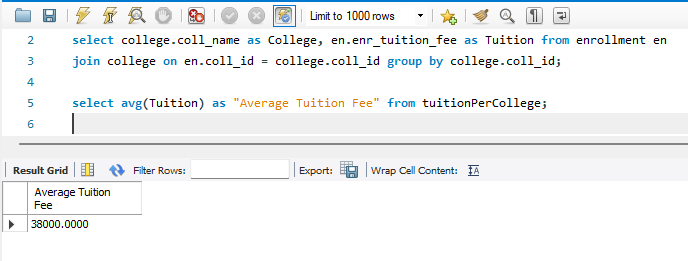
\includegraphics[width=0.7\linewidth]{images/q1.png}
    \caption{Question 1 Query and Output}
\end{figure}
